\documentclass[12pt]{article}
\usepackage{amsmath}
\usepackage{amsfonts}
\usepackage{graphicx}
\usepackage{subcaption}
\usepackage{url}
\usepackage{siunitx}
\usepackage{listings}
\usepackage{color} %red, green, blue, yellow, cyan, magenta, black, white
\definecolor{mygreen}{RGB}{28,172,0} % color values Red, Green, Blue
\definecolor{mylilas}{RGB}{170,55,241}
\setlength{\oddsidemargin}{0in}
\setlength{\evensidemargin}{0in}
\setlength{\textheight}{9in}
\setlength{\textwidth}{6.5in}
\setlength{\topmargin}{-0.5in}

\title{\bf Assignment 2 \\[2ex] 
	\rm\normalsize Solid State Physics}
\date{\today}
\author{\bf Declan Mathews [s1610357][B103565]}

\begin{document}
	\maketitle
	\section{Problem 1: Equation of State of Iridium Metal}
			\begin{figure}[h!!!!!]
				\centering
				\begin{subfigure}[t]{0.5\textwidth}
					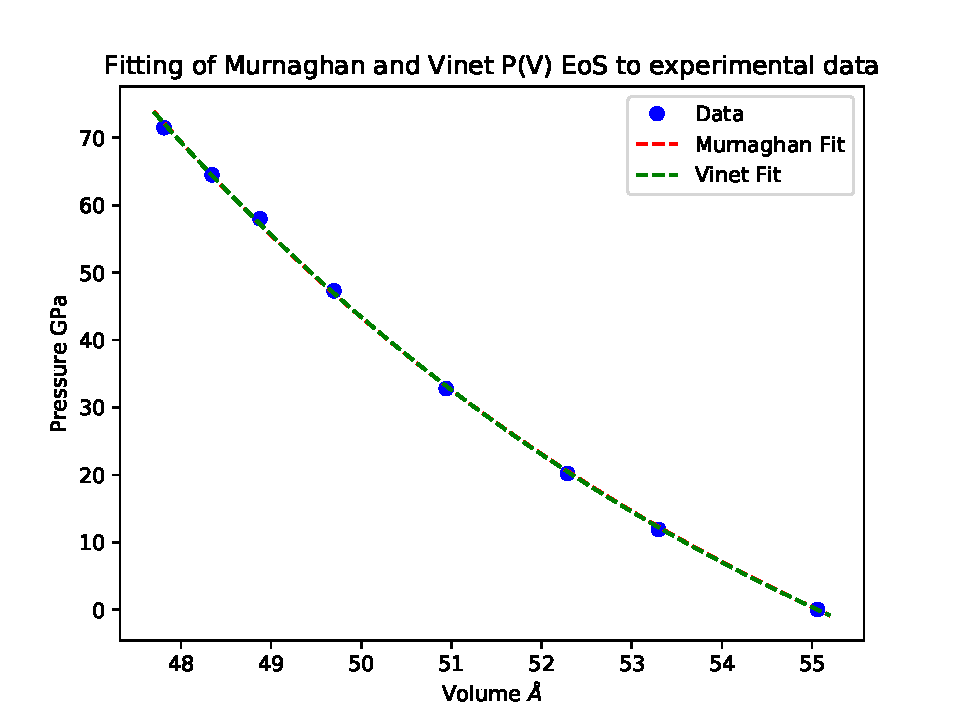
\includegraphics[width=8cm]{../PVfits}
					\subcaption{Fitting of the Murnaghan and Vinet\\$P(V)$ equations of state to the experimental\\data. Note that they are mostly superimposed.}
					\label{fig:EoSa}
				\end{subfigure}%
				\begin{subfigure}[t]{0.5\textwidth}
					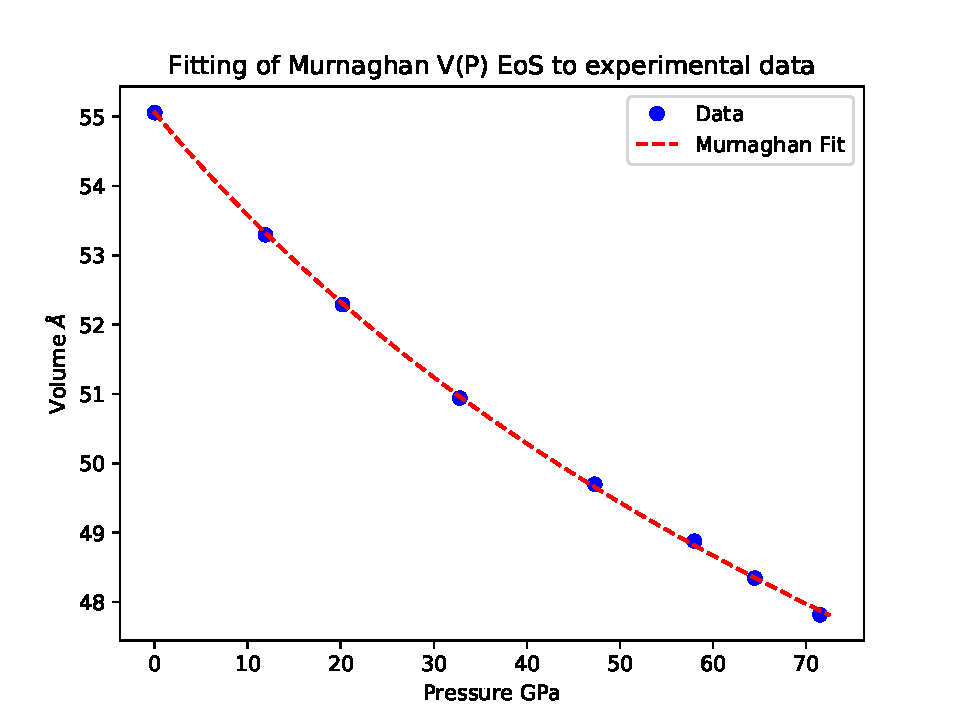
\includegraphics[width=8cm]{../VPfit}
					\subcaption{Fitting of the Murnaghan $V(P)$ equation of state to the experimental data.}
					\label{fig:EoSb}
				\end{subfigure}
				\caption{The equation of state fits to the supplied data.}
				\label{fig:EoS}
			\end{figure}
		
		
		\begin{table}[h!!!]
			\centering
			\begin{tabular}{l|l|l|ll}
				\cline{2-3}
				& $B_0$ /\SI{}{\GPa}                 & $B_0^{\prime}$ /\SI{}{\GPa}            &  &  \\ \cline{1-3}
				\multicolumn{1}{|l|}{Murnaghan P(V)} & 346.608351 ($\pm 2.15\%$) & 5.19847436 ($\pm 6.05\%$) &  &  \\ \cline{1-3}
				\multicolumn{1}{|l|}{Vinet P(V)}     & 341.136046 ($\pm 2.12\%$) & 5.84136407 ($\pm 6.00\%$) &  &  \\ \cline{1-3}
				\multicolumn{1}{|l|}{Murnaghan V(P)} & 340.792229 ($\pm 1.74\%$) & 5.45810675 ($\pm 4.91\%$) &  &  \\ \cline{1-3}
			\end{tabular}
			\caption{The results and their errors from the fits. $V_0$ is not varied as a parameter and set as the recorded zero pressure volume of $55.059 \AA^3$.}
			\label{tab:results}
		\end{table}
	
	\newpage
	\noindent Using the module \texttt{lmfit}, the Murnaghan $P(V)$, Vinet $P(V)$ and Murnaghan $V(P)$ were fit to the supplied data, as shown in Figure \ref{fig:EoS}. The initial volume $V_0$ was not varied as a parameter but was given as the experimental volume result at zero pressure ($55.059 \AA^3$). The results from the fitting of each equation of state for $B_0$ and $B_0^{\prime}$ are shown with percentage errors in Table \ref{tab:results}. $V_0$ was chosen as a constant value as theoretically a pure unit cell of Iridium would have a fixed volume at zero pressure. In practice, this could vary very slightly. However, when performing fits, more accurate results are achieved with less fitting parameters. On top of this, the data provides a measured value at zero pressure and so keeping that fixed constrains the analysis to studying the particular system based on the gathered results.
	
	\bigskip
	
	\noindent Based on the results, the Vinet $P(V)$ method appears to fit better than the Murnaghan $P(V)$ method. This is due to the smaller percentage errors on both $B_0$ and $B_0^{\prime}$, suggesting less variation of the data from the fit line.
	
	\bigskip
	
	\noindent The Murnaghan $V(P)$ fit is in good agreement with the $P(V)$ fit. They both give $B_0 \approx 340 GPa$ and $B_0^{\prime} \approx 5 GPa$. The $V(P)$ fit also has much smaller percantage errors than the two $P(V)$ fits. However, the value for $B_0$ is much closer to the Vinet result (and the $B_0^{\prime}$ value is roughly in the middle).  As the Vinet fit is in closer agreement with another even smaller percentage error fit it suggests further that Vinet $P(V)$ is a 'better' fit than Murnaghan $P(V)$.
	
	\bigskip
	
	\noindent From these results, $B_0 = $ \SI{340.79}{\GPa} and $B_0^{\prime} = $ \SI{5.46}{\GPa}. The experimental value of the bulk modulus is given as $B = $ \SI{320}{\GPa}.\footnote{As seen at https://www.webelements.com/iridium/physics.html} This is approximately the result achieved from this analysis as it is within 10\%.
	
	
	\section{Problem 2: DFT}
		\subsection*{Generalised Gradient Approximation (GGA)}
		This is a method of approximating the unknown exhange-correlation functional. It builds on the Local Density Approximation (LDA) method by introducing some non-locality in the form of the gradient of the electron density, as well as the electron density itself, at each point in the unit cell. It is given by the equation:
		
		\begin{equation}
		E_{XC}^{GGA}[\rho] = \int \epsilon_{XC}^{\prime}(\rho, \nabla\rho)\cdot\rho(\textbf{r}) dV
		\end{equation}
		Where $\rho$ is the electron density and $\nabla\rho$ is the electron density gradient.

		\subsection*{Born-Oppenheimer approximation}
		The electron and nuclei are assumed to have independent motions. This is substatiated by the mass of a nucleus being significantly higher than the mass of an electron. By the classical equipartition theorem we expect the kinetic energies to be equal and so the electron moves much faster than the nuclei to an extent at which the nuclei can be considered stationary. The kintetic energies and interaction potentials can then be calculated seperately, by classical methods for the nuclei and quantum mechinically for the electrons.

		\subsection*{Kohn-Sham equation}
		This equation is:
		\begin{equation}
		[\hat{T} + V_{eff}]\psi_i(\textbf{r}) = \epsilon_i \psi_i(\textbf{r})
		\end{equation}
		Where $V_{eff}(\textbf{r}) = V_{ne}(\textbf{r}) + V_{ee}(\textbf{r}) + V_{xc}(\textbf{r})$
		
		\bigskip
		
		\noindent Here, $\hat{T}$ is the kinetic energy operator, $V_{eff}$ is the effective potential (a summation of the nucleus-electron, electron-electron and exchange-correlation potential) and $\epsilon_i$ and $\psi_i(\textbf{r})$ are the single-electron energy eigenvalues and wavefunctions.
		
		\bigskip
		
		\noindent This equation describes a fictitious system of non-interacting electrons ($i$ is the elctron index) which can be used to produce the true ground state electron density of the fully interacting system using the equation:
		
		\begin{equation}
		\rho(\textbf{r}) = \sum_{i, occ.}^{}|\psi_i(\textbf{r})|^2
		\end{equation}
		Where the sum is over all occupied states.
	
		\bigskip
		
		\noindent This equation is part of a self-consistent loop in DFT calculations to calculate the true ground state electron density by looking for convergence in the total energy at each iteration. This electron density describes the wavefunction and allows the energy of the system to be calculated.

		\subsection*{Pseudopotential}
		There are rapid flucuations of the true electron wavefunctions near the core of atoms. This requires many plane waves to describe accurately which is very computationally expensive. This also occurs in the region which is much less relevant for DFT calculations. As this region is not very relevant, it can be replaced by smooth pre-calulcated pseudopotentials without much loss in accuracy of the DFT calculations. The plane wave expansion is then only used in the more well behaved and relevant areas further from the nucleus centre resulting is cheaper computational calculations.
		
	
\end{document}